\documentclass[../main.tex]{subfiles}

\begin{document}
\begin{problema}[3]
	Investigar y describir la información que se pide en los siguientes incisos.
	Anotar la referencia bibliográfica de donde se obtuvo la información.

	\begin{enumerate}
		\item ¿Qué es el módulo de Young?
		\item ¿Cuál es la diferencia entre el módulo de Young y el módulo
		      de cizalla?
		\item Describe cómo se puede medir el módulo de Young experimentalmente.
		\item Enlista el valor del número de Young de tres materiales diferentes.
		\item ¿Qué es el efecto Poisson en elasticidad?
		\item Dar un ejemplo de un material que muestre una respuesta opuesta
		      al efecto Poisson al aplicarle una compresión/estiramiento.
	\end{enumerate}

	\startsolution

	\section{Inciso (a)}

	El módulo de Young es una constante numérica que se utiliza para describir las
	propiedades elásticas de un material sólido, como una barra de metal, que se somete
	a fuerzas de tensión o compresión. Mide la capacidad de una muestra para soportar
	cambios de longitud y solo es relevante cuando la tensión (carga) es proporcional a
	la deformación (elongación).\cite{PruebaModuloYoungs2022}

	\section{Inciso (b)}

	La diferencia entre el módulo de Young y el módulo de cizalla radica en que el primero
	mide la resistencia a los cambios de longitud bajo tensión o compresión, mientras que
	el segundo evalúa la rigidez de un material sometido a esfuerzos cortantes.\cite{ModuloElasticidadQue2022}

	\section{Inciso (c)}

	La medición del módulo de Young se puede realizar mediante una prueba de tracción (ASTM D638 o ISO 527-1). Para esta prueba, la muestra se extiende a lo largo de su eje longitudinal
	a una velocidad constante hasta que se fracture o hasta que la tensión (carga) aplicada o la
	deformación (elongación) alcance un valor predeterminado. Durante esta prueba, se miden
	la carga soportada por la prueba y su elongación. El módulo de Young se obtiene a partir
	del gradiente de la curva en el gradiente de tensión-deformación, en particular de la
	región de elasticidad lineal.\cite{ASTMD638Caracteristicas,LordYounModulus,ISO527}

	\section{Inciso (d)}

	En la siguiente tabla se muestran algunos valores del módulo de Young,

	\begin{table}[htb]
		\centering
		\begin{tblr}{
				colspec = cc,
				hlines,
				row{1} = {font=\bfseries},
				vlines,
			}
			Material & Módulo de Young (\unit{\GPa})            \\
			Aluminio & \numrange[range-phrase=--]{68.2}{78.5}   \\
			Cobre    & \numrange[range-phrase=--]{117}{124}     \\
			Titanio  & \numrange[range-phrase=--]{106.1}{114.4} \\
		\end{tblr}
		\caption{Valor del módulo de Young para distintos materiales.\cite{Lai-Continuum}}
	\end{table}
	\section{Inciso (e)}

	El efecto de Poisson en elasticidad se refiere a que, cuando un material se somete a
	una tracción (compresión), simultáneamente se contrae (expande) en la dirección perpendicular
	a la carga aplicada \cite{graffChapter6Power2023} (véase \zcref{fig:poisson-effect}).

	\begin{figure}[htb]
		\centering
		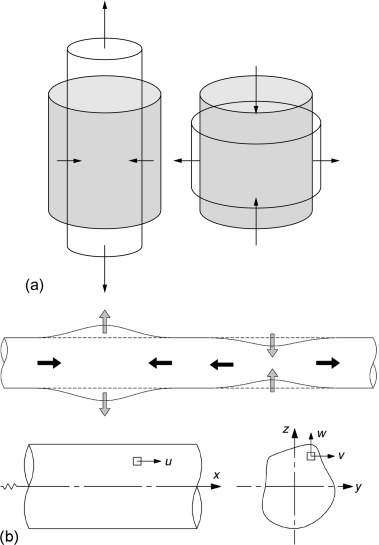
\includegraphics[scale=0.6]{figs/poisson.jpg}
		\caption{Efecto de Poisson en vibraciones: (a) Efecto de Poisson: (b) expansión, contracción perpendicular debido al efecto de Poisson.\cite{graffChapter6Power2023}}
		\label{fig:poisson-effect}
	\end{figure}

	\section{Inciso (f)}

	Que un material muestre una respuesta opuesta al efecto Poisson significa que,
	cuando se somete a una tracción, se expande en la dirección transversal, mientras
	que se contrae bajo compresión. A este tipo de materiales se les denomina
	materiales auxéticos.
	Un ejemplo de este tipo de materiales son las espumas de poliuretanos.\cite{LiAuxeticPUFoam2016}

\end{problema}
\end{document}
